% Created 2025-01-12 Sun 19:09
% Intended LaTeX compiler: pdflatex
\documentclass[11pt]{article}
\usepackage[utf8]{inputenc}
\usepackage[T1]{fontenc}
\usepackage{graphicx}
\usepackage{longtable}
\usepackage{wrapfig}
\usepackage{rotating}
\usepackage[normalem]{ulem}
\usepackage{amsmath}
\usepackage{amssymb}
\usepackage{capt-of}
\usepackage{hyperref}
\usepackage[polish]{babel}
\usepackage[T1]{fontenc}
\usepackage[utf8]{inputenc}
\selectlanguage{polish}
\usepackage{caption}
\usepackage{booktabs}
\captionsetup{labelfont=bf}
\usepackage{float}
\usepackage{svg}
\usepackage[a4paper, total={7.0in, 10.2in}]{geometry}
\author{Piotr Karamon}
\date{13.01.2025.}
\title{Laboratorium 10 cz. 2 - Teoria śladów}
\hypersetup{
 pdfauthor={Piotr Karamon},
 pdftitle={Laboratorium 10 cz. 2 - Teoria śladów},
 pdfkeywords={},
 pdfsubject={},
 pdfcreator={Emacs 29.2 (Org mode 9.7.11)}, 
 pdflang={Polish}}

% Setup for code blocks [1/2]

\usepackage{fvextra}

\fvset{%
  commandchars=\\\{\},
  highlightcolor=white!95!black!80!blue,
  breaklines=true,
  breaksymbol=\color{white!60!black}\tiny\ensuremath{\hookrightarrow}}

% Make line numbers smaller and grey.
\renewcommand\theFancyVerbLine{\footnotesize\color{black!40!white}\arabic{FancyVerbLine}}

\usepackage{xcolor}

% In case engrave-faces-latex-gen-preamble has not been run.
\providecolor{EfD}{HTML}{f7f7f7}
\providecolor{EFD}{HTML}{28292e}

% Define a Code environment to prettily wrap the fontified code.
\usepackage[breakable,xparse]{tcolorbox}
\DeclareTColorBox[]{Code}{o}%
{colback=EfD!98!EFD, colframe=EfD!95!EFD,
  fontupper=\footnotesize\setlength{\fboxsep}{0pt},
  colupper=EFD,
  IfNoValueTF={#1}%
  {boxsep=2pt, arc=2.5pt, outer arc=2.5pt,
    boxrule=0.5pt, left=2pt}%
  {boxsep=2.5pt, arc=0pt, outer arc=0pt,
    boxrule=0pt, leftrule=1.5pt, left=0.5pt},
  right=2pt, top=1pt, bottom=0.5pt,
  breakable}

% Support listings with captions
\usepackage{float}
\floatstyle{plain}
\newfloat{listing}{htbp}{lst}
\newcommand{\listingsname}{Listing}
\floatname{listing}{\listingsname}
\newcommand{\listoflistingsname}{List of Listings}
\providecommand{\listoflistings}{\listof{listing}{\listoflistingsname}}


% Setup for code blocks [2/2]: syntax highlighting colors

\newcommand\efstrut{\vrule height 2.1ex depth 0.8ex width 0pt}
\definecolor{EFD}{HTML}{000000}
\definecolor{EfD}{HTML}{ffffff}
\newcommand{\EFD}[1]{\textcolor{EFD}{#1}} % default
\newcommand{\EFvp}[1]{#1} % variable-pitch
\definecolor{EFh}{HTML}{595959}
\newcommand{\EFh}[1]{\textcolor{EFh}{#1}} % shadow
\definecolor{EFsc}{HTML}{005f5f}
\newcommand{\EFsc}[1]{\textcolor{EFsc}{\textbf{#1}}} % success
\definecolor{EFw}{HTML}{884900}
\newcommand{\EFw}[1]{\textcolor{EFw}{\textbf{#1}}} % warning
\definecolor{EFe}{HTML}{a60000}
\newcommand{\EFe}[1]{\textcolor{EFe}{\textbf{#1}}} % error
\definecolor{EFl}{HTML}{3548cf}
\newcommand{\EFl}[1]{\textcolor{EFl}{#1}} % link
\definecolor{EFlv}{HTML}{721045}
\newcommand{\EFlv}[1]{\textcolor{EFlv}{#1}} % link-visited
\definecolor{Efhi}{HTML}{b2e4dc}
\newcommand{\EFhi}[1]{\colorbox{Efhi}{\efstrut{}#1}} % highlight
\definecolor{EFc}{HTML}{595959}
\newcommand{\EFc}[1]{\textcolor{EFc}{\textit{#1}}} % font-lock-comment-face
\definecolor{EFcd}{HTML}{595959}
\newcommand{\EFcd}[1]{\textcolor{EFcd}{\textit{#1}}} % font-lock-comment-delimiter-face
\definecolor{EFs}{HTML}{3548cf}
\newcommand{\EFs}[1]{\textcolor{EFs}{#1}} % font-lock-string-face
\definecolor{EFd}{HTML}{2a5045}
\newcommand{\EFd}[1]{\textcolor{EFd}{\textit{#1}}} % font-lock-doc-face
\definecolor{EFm}{HTML}{7c318f}
\newcommand{\EFm}[1]{\textcolor{EFm}{\textit{#1}}} % font-lock-doc-markup-face
\definecolor{EFk}{HTML}{531ab6}
\newcommand{\EFk}[1]{\textcolor{EFk}{#1}} % font-lock-keyword-face
\definecolor{EFb}{HTML}{8f0075}
\newcommand{\EFb}[1]{\textcolor{EFb}{#1}} % font-lock-builtin-face
\definecolor{EFf}{HTML}{721045}
\newcommand{\EFf}[1]{\textcolor{EFf}{#1}} % font-lock-function-name-face
\definecolor{EFv}{HTML}{005e8b}
\newcommand{\EFv}[1]{\textcolor{EFv}{#1}} % font-lock-variable-name-face
\definecolor{EFt}{HTML}{005f5f}
\newcommand{\EFt}[1]{\textcolor{EFt}{#1}} % font-lock-type-face
\definecolor{EFo}{HTML}{0000b0}
\newcommand{\EFo}[1]{\textcolor{EFo}{#1}} % font-lock-constant-face
\definecolor{EFwr}{HTML}{884900}
\newcommand{\EFwr}[1]{\textcolor{EFwr}{#1}} % font-lock-warning-face
\definecolor{EFnc}{HTML}{a60000}
\newcommand{\EFnc}[1]{\textcolor{EFnc}{\textbf{#1}}} % font-lock-negation-char-face
\definecolor{EFpp}{HTML}{a0132f}
\newcommand{\EFpp}[1]{\textcolor{EFpp}{#1}} % font-lock-preprocessor-face
\definecolor{EFrc}{HTML}{00663f}
\newcommand{\EFrc}[1]{\textcolor{EFrc}{#1}} % font-lock-regexp-grouping-construct
\definecolor{EFrb}{HTML}{721045}
\newcommand{\EFrb}[1]{\textcolor{EFrb}{#1}} % font-lock-regexp-grouping-backslash
\definecolor{Efob}{HTML}{f2f2f2}
\newcommand{\EFob}[1]{\colorbox{Efob}{\efstrut{}#1}} % org-block
\definecolor{EFobb}{HTML}{595959}
\definecolor{Efobb}{HTML}{f2f2f2}
\newcommand{\EFobb}[1]{\colorbox{Efobb}{\efstrut{}\textcolor{EFobb}{#1}}} % org-block-begin-line
\definecolor{EFobe}{HTML}{595959}
\definecolor{Efobe}{HTML}{f2f2f2}
\newcommand{\EFobe}[1]{\colorbox{Efobe}{\efstrut{}\textcolor{EFobe}{#1}}} % org-block-end-line
\newcommand{\EFOa}[1]{\textbf{#1}} % outline-1
\definecolor{EFOb}{HTML}{624416}
\newcommand{\EFOb}[1]{\textcolor{EFOb}{\textbf{#1}}} % outline-2
\definecolor{EFOc}{HTML}{193668}
\newcommand{\EFOc}[1]{\textcolor{EFOc}{\textbf{#1}}} % outline-3
\definecolor{EFOd}{HTML}{721045}
\newcommand{\EFOd}[1]{\textcolor{EFOd}{\textbf{#1}}} % outline-4
\definecolor{EFOe}{HTML}{2a5045}
\newcommand{\EFOe}[1]{\textcolor{EFOe}{\textbf{#1}}} % outline-5
\definecolor{EFOf}{HTML}{7f0000}
\newcommand{\EFOf}[1]{\textcolor{EFOf}{\textbf{#1}}} % outline-6
\definecolor{EFOg}{HTML}{3f578f}
\newcommand{\EFOg}[1]{\textcolor{EFOg}{\textbf{#1}}} % outline-7
\definecolor{EFOh}{HTML}{595959}
\newcommand{\EFOh}[1]{\textcolor{EFOh}{\textbf{#1}}} % outline-8
\definecolor{EFhn}{HTML}{0000b0}
\newcommand{\EFhn}[1]{\textcolor{EFhn}{#1}} % highlight-numbers-number
\newcommand{\EFhq}[1]{#1} % highlight-quoted-quote
\newcommand{\EFhs}[1]{#1} % highlight-quoted-symbol
\newcommand{\EFrda}[1]{#1} % rainbow-delimiters-depth-1-face
\definecolor{EFrdb}{HTML}{dd22dd}
\newcommand{\EFrdb}[1]{\textcolor{EFrdb}{#1}} % rainbow-delimiters-depth-2-face
\definecolor{EFrdc}{HTML}{008899}
\newcommand{\EFrdc}[1]{\textcolor{EFrdc}{#1}} % rainbow-delimiters-depth-3-face
\definecolor{EFrdd}{HTML}{972500}
\newcommand{\EFrdd}[1]{\textcolor{EFrdd}{#1}} % rainbow-delimiters-depth-4-face
\definecolor{EFrde}{HTML}{808000}
\newcommand{\EFrde}[1]{\textcolor{EFrde}{#1}} % rainbow-delimiters-depth-5-face
\definecolor{EFrdf}{HTML}{531ab6}
\newcommand{\EFrdf}[1]{\textcolor{EFrdf}{#1}} % rainbow-delimiters-depth-6-face
\definecolor{EFrdg}{HTML}{008900}
\newcommand{\EFrdg}[1]{\textcolor{EFrdg}{#1}} % rainbow-delimiters-depth-7-face
\definecolor{EFrdh}{HTML}{3548cf}
\newcommand{\EFrdh}[1]{\textcolor{EFrdh}{#1}} % rainbow-delimiters-depth-8-face
\definecolor{EFrdi}{HTML}{8f0075}
\newcommand{\EFrdi}[1]{\textcolor{EFrdi}{#1}} % rainbow-delimiters-depth-9-face
\definecolor{EFany}{HTML}{6f5500}
\definecolor{Efany}{HTML}{6f5500}
\newcommand{\EFany}[1]{\colorbox{Efany}{\efstrut{}\textcolor{EFany}{#1}}} % ansi-color-yellow
\definecolor{EFanr}{HTML}{a60000}
\definecolor{Efanr}{HTML}{a60000}
\newcommand{\EFanr}[1]{\colorbox{Efanr}{\efstrut{}\textcolor{EFanr}{#1}}} % ansi-color-red
\definecolor{EFanb}{HTML}{000000}
\definecolor{Efanb}{HTML}{000000}
\newcommand{\EFanb}[1]{\colorbox{Efanb}{\efstrut{}\textcolor{EFanb}{#1}}} % ansi-color-black
\definecolor{EFang}{HTML}{006800}
\definecolor{Efang}{HTML}{006800}
\newcommand{\EFang}[1]{\colorbox{Efang}{\efstrut{}\textcolor{EFang}{#1}}} % ansi-color-green
\definecolor{EFanB}{HTML}{0031a9}
\definecolor{EfanB}{HTML}{0031a9}
\newcommand{\EFanB}[1]{\colorbox{EfanB}{\efstrut{}\textcolor{EFanB}{#1}}} % ansi-color-blue
\definecolor{EFanc}{HTML}{005e8b}
\definecolor{Efanc}{HTML}{005e8b}
\newcommand{\EFanc}[1]{\colorbox{Efanc}{\efstrut{}\textcolor{EFanc}{#1}}} % ansi-color-cyan
\definecolor{EFanw}{HTML}{a6a6a6}
\definecolor{Efanw}{HTML}{a6a6a6}
\newcommand{\EFanw}[1]{\colorbox{Efanw}{\efstrut{}\textcolor{EFanw}{#1}}} % ansi-color-white
\definecolor{EFanm}{HTML}{721045}
\definecolor{Efanm}{HTML}{721045}
\newcommand{\EFanm}[1]{\colorbox{Efanm}{\efstrut{}\textcolor{EFanm}{#1}}} % ansi-color-magenta
\definecolor{EFANy}{HTML}{884900}
\definecolor{EfANy}{HTML}{884900}
\newcommand{\EFANy}[1]{\colorbox{EfANy}{\efstrut{}\textcolor{EFANy}{#1}}} % ansi-color-bright-yellow
\definecolor{EFANr}{HTML}{972500}
\definecolor{EfANr}{HTML}{972500}
\newcommand{\EFANr}[1]{\colorbox{EfANr}{\efstrut{}\textcolor{EFANr}{#1}}} % ansi-color-bright-red
\definecolor{EFANb}{HTML}{595959}
\definecolor{EfANb}{HTML}{595959}
\newcommand{\EFANb}[1]{\colorbox{EfANb}{\efstrut{}\textcolor{EFANb}{#1}}} % ansi-color-bright-black
\definecolor{EFANg}{HTML}{00663f}
\definecolor{EfANg}{HTML}{00663f}
\newcommand{\EFANg}[1]{\colorbox{EfANg}{\efstrut{}\textcolor{EFANg}{#1}}} % ansi-color-bright-green
\definecolor{EFANB}{HTML}{3548cf}
\definecolor{EfANB}{HTML}{3548cf}
\newcommand{\EFANB}[1]{\colorbox{EfANB}{\efstrut{}\textcolor{EFANB}{#1}}} % ansi-color-bright-blue
\definecolor{EFANc}{HTML}{005f5f}
\definecolor{EfANc}{HTML}{005f5f}
\newcommand{\EFANc}[1]{\colorbox{EfANc}{\efstrut{}\textcolor{EFANc}{#1}}} % ansi-color-bright-cyan
\definecolor{EFANw}{HTML}{ffffff}
\definecolor{EfANw}{HTML}{ffffff}
\newcommand{\EFANw}[1]{\colorbox{EfANw}{\efstrut{}\textcolor{EFANw}{#1}}} % ansi-color-bright-white
\definecolor{EFANm}{HTML}{531ab6}
\definecolor{EfANm}{HTML}{531ab6}
\newcommand{\EFANm}[1]{\colorbox{EfANm}{\efstrut{}\textcolor{EFANm}{#1}}} % ansi-color-bright-magenta
\begin{document}

\maketitle
\section*{Treść zadania}
\label{sec:orgf97f338}
Dane są:
\begin{itemize}
\item Alfabet \(A\), w którym każda litera oznacza akcje.
\item Relacja niezależności \(I\), oznaczająca które akcje są niezależne (przemienne,
tzn. można je wykonać w dowolnej kolejności i nie zmienia to wyniku końcowego).
\item Słowo \(w\) oznaczające przykładowe wykonanie sekwencji akcji.
\end{itemize}



Napisz program w dowolnym języku, który:
\begin{enumerate}
\item Wyznacza relację niezależności \(I\)
\item Wyznacza ślad \([w]\) względem relacji I
\item Wyznacza postać normalną na Foaty \(\text{FNF}([w])\) śladu \([w]\)
\item Wyznacza graf zależności dla słowa \(w\)
\item Wyznacza postać normalną Foaty na podstawie grafu
\end{enumerate}
\section*{Rozwiązanie}
\label{sec:orgf45434e}
Kod został napisany w języku Java.
Klasą która rozwiązuje zadane problemy jest \texttt{TraceSolver}. Otrzymuje na wejściu alfabet,
zbiór par informujących o tym, które akcje są niezależne oraz słowo.
\begin{Code}
\begin{Verbatim}
\color{EFD}\EFt{record} \EFf{Pair}\EFrda{(}\EFt{char} \EFv{a}, \EFt{char} \EFv{b}\EFrda{)} \EFrda{\{}
    \textcolor[HTML]{0000b0}{@Override}
    \EFk{public} \EFt{String} \EFf{toString}\EFrdb{(}\EFrdb{)} \EFrdb{\{}
        \EFk{return} \EFs{"(\%s, \%s)"}.formatted\EFrdc{(}a, b\EFrdc{)};
    \EFrdb{\}}
\EFrda{\}}
\EFk{class} \EFt{TraceSolver} \EFrda{\{}
    \EFk{private} \EFk{final} \EFt{Set}\EFrdb{<}\EFt{Character}\EFrdb{>} \EFv{alphabet};
    \EFk{private} \EFk{final} \EFt{Set}\EFrdb{<}\EFt{Pair}\EFrdb{>} \EFv{independenceRelation};
    \EFk{private} \EFk{final} \EFt{Set}\EFrdb{<}\EFt{Pair}\EFrdb{>} \EFv{dependenceRelation};
    \EFk{private} \EFk{final} \EFt{String} \EFv{word};

    \EFk{public} TraceSolver\EFrdb{(}\EFt{Set}\EFrdc{<}\EFt{Character}\EFrdc{>} \EFv{alphabet},
                       \EFt{Set}\EFrdc{<}\EFt{Pair}\EFrdc{>} \EFv{independentPairs},
                       String word

    \EFrdb{)} \EFrdb{\{}
        \EFk{this}.alphabet = alphabet;
        \EFk{this}.independenceRelation = computeIndependenceRelation\EFrdc{(}independentPairs\EFrdc{)};
        \EFk{this}.dependenceRelation = computeDependenceRelation\EFrdc{(}independenceRelation\EFrdc{)};
        \EFk{this}.word = word;
    \EFrdb{\}}
\EFrda{\}}
\end{Verbatim}
\end{Code}
\subsection*{Wyznaczenie relacji niezależności i zależności}
\label{sec:org38fc181}
Relację niezależności otrzymujemy poprzez stworzenie zbioru, który zawiera pary \((a,b)\), \((b,a)\)
dla każdej takiej pary w \texttt{independentPairs.}

\begin{Code}
\begin{Verbatim}
\color{EFD}\EFk{private} \EFk{static} \EFt{Set}\EFrda{<}\EFt{Pair}\EFrda{>} \EFf{computeIndependenceRelation}\EFrda{(}\EFt{Set}\EFrdb{<}\EFt{Pair}\EFrdb{>} \EFv{independentPairs}\EFrda{)} \EFrda{\{}
    \EFk{return} independentPairs
            .stream\EFrdb{(}\EFrdb{)}
            .flatMap\EFrdb{(}
                    pair -> Stream.of\EFrdc{(}\EFk{new} \EFt{Pair}\EFrdd{(}pair.a\EFrda{(}\EFrda{)}, pair.b\EFrda{(}\EFrda{)}\EFrdd{)}, \EFk{new} \EFt{Pair}\EFrdd{(}pair.b\EFrda{(}\EFrda{)}, pair.a\EFrda{(}\EFrda{)}\EFrdd{)}\EFrdc{)}
            \EFrdb{)}
            .collect\EFrdb{(}Collectors.toSet\EFrdc{(}\EFrdc{)}\EFrdb{)};
\EFrda{\}}

\EFk{public} \EFt{Set}\EFrda{<}\EFt{Pair}\EFrda{>} \EFf{getIndependenceRelation}\EFrda{(}\EFrda{)} \EFrda{\{}
    \EFk{return} independenceRelation;
\EFrda{\}}
\end{Verbatim}
\end{Code}

Relację zależności tworzymy iterując po wszystkich parach \((a,b) \in A^2\), sprawdzamy
czy para ta nie należy do \(I\), jeżeli tak to należy ona do \(D\) i dodajemy ją do tworzonego zbioru.

\begin{Code}
\begin{Verbatim}
\color{EFD}\EFk{private} \EFt{Set}\EFrda{<}\EFt{Pair}\EFrda{>} \EFf{computeDependenceRelation}\EFrda{(}\EFt{Set}\EFrdb{<}\EFt{Pair}\EFrdb{>} \EFv{independentRelation}\EFrda{)} \EFrda{\{}
    \EFt{Set}\EFrdb{<}\EFt{Pair}\EFrdb{>} \EFv{dependenceRelation} = \EFk{new} \EFt{HashSet}\EFrdb{<}\EFrdb{>}\EFrdb{(}\EFrdb{)};
    \EFk{for} \EFrdb{(}\EFt{char} \EFv{a} : alphabet\EFrdb{)} \EFrdb{\{}
        \EFk{for} \EFrdc{(}\EFt{char} \EFv{b} : alphabet\EFrdc{)} \EFrdc{\{}
            \EFt{Pair} \EFv{pair} = \EFk{new} \EFt{Pair}\EFrdd{(}a, b\EFrdd{)};
            \EFk{if} \EFrdd{(}\EFnc{!}independentRelation.contains\EFrda{(}pair\EFrda{)}\EFrdd{)} \EFrdd{\{}
                dependenceRelation.add\EFrda{(}pair\EFrda{)};
            \EFrdd{\}}
        \EFrdc{\}}
    \EFrdb{\}}

    \EFk{return} dependenceRelation;
\EFrda{\}}

\EFk{public} \EFt{Set}\EFrda{<}\EFt{Pair}\EFrda{>} \EFf{getDependenceRelation}\EFrda{(}\EFrda{)} \EFrda{\{}
    \EFk{return} dependenceRelation;
\EFrda{\}}
\end{Verbatim}
\end{Code}
\subsection*{Wyznaczanie śladu \([w]\)}
\label{sec:orgcc4ff92}
Używamy następującego algorytmu:
\begin{enumerate}
\item Tworzymy zbiór \texttt{trace} i dodajemy do niego słowo \(w\).
\item Próbujemy powiększyć zbiór \texttt{trace} dodając do niego wyrazy, które powstały w wyniku
zamiany dwóch sąsiednich liter, które są niezależne.
\begin{enumerate}
\item Tworzymy zbiór \texttt{newTrace}
\item Dla każdego wyrazu w \texttt{trace}:
\begin{enumerate}
\item Dodajemy go do \texttt{newTrace}
\item Przechodzimy przez wyraz i jeżeli dwie litery obok siebie są niezależne,
to zamieniamy je miejscami i dodajemy je do \texttt{newTrace}
\end{enumerate}
\item Jeżeli \texttt{newTrace = trace} to oznacza, że kończymy. Jeżeli jest to fałsz to znów
próbujemy powiększyć \texttt{trace}
\end{enumerate}
\end{enumerate}
\newpage

\begin{Code}
\begin{Verbatim}
\color{EFD}\EFk{public} \EFt{Set}\EFrda{<}\EFt{String}\EFrda{>} \EFf{getTrace}\EFrda{(}\EFrda{)} \EFrda{\{}
    \EFt{Set}\EFrdb{<}\EFt{String}\EFrdb{>} \EFv{trace} = \EFk{new} \EFt{HashSet}\EFrdb{<}\EFrdb{>}\EFrdb{(}\EFrdb{)};
    trace.add\EFrdb{(}word\EFrdb{)};

    \EFk{while} \EFrdb{(}\EFo{true}\EFrdb{)} \EFrdb{\{}
        \EFt{Set}\EFrdc{<}\EFt{String}\EFrdc{>} \EFv{newTrace} = \EFk{new} \EFt{HashSet}\EFrdc{<}\EFrdc{>}\EFrdc{(}\EFrdc{)};

        \EFk{for} \EFrdc{(}\EFt{String} \EFv{word} : trace\EFrdc{)} \EFrdc{\{}
            newTrace.add\EFrdd{(}word\EFrdd{)};
            \EFk{for} \EFrdd{(}\EFt{int} \EFv{i} = \EFhn{0}; i < word.\EFt{length}\EFrda{(}\EFrda{)} - \EFhn{1}; i++\EFrdd{)} \EFrdd{\{}
                \EFt{char} \EFv{a} = word.charAt\EFrda{(}i\EFrda{)};
                \EFt{char} \EFv{b} = word.charAt\EFrda{(}i + \EFhn{1}\EFrda{)};
                \EFt{Pair} \EFv{pair} = \EFk{new} \EFt{Pair}\EFrda{(}a, b\EFrda{)};
                \EFk{if} \EFrda{(}independenceRelation.contains\EFrdb{(}pair\EFrdb{)}\EFrda{)} \EFrda{\{}
                    \EFt{String} \EFv{newWord} = word.substring\EFrdb{(}\EFhn{0}, i\EFrdb{)} + b + a + word.substring\EFrdb{(}i + \EFhn{2}\EFrdb{)};
                    newTrace.add\EFrdb{(}newWord\EFrdb{)};
                \EFrda{\}}
            \EFrdd{\}}
        \EFrdc{\}}
        \EFk{if} \EFrdc{(}newTrace.equals\EFrdd{(}trace\EFrdd{)}\EFrdc{)} \EFrdc{\{}
            \EFk{break};
        \EFrdc{\}}
        trace = newTrace;
    \EFrdb{\}}
    \EFk{return} trace;
\EFrda{\}}
\end{Verbatim}
\end{Code}
\subsection*{Wyznaczanie postaci normalnej Foaty}
\label{sec:org0ea4b8b}
Algorytm:
\begin{enumerate}
\item Dla każdej litery \(a \in A\) tworzymy stos.
\item Przechodzimy przez wyraz \(w\) od prawej do lewej:
\begin{enumerate}
\item Dodajemy literę na odpowiadający jej stos.
\item Dla wszystkich \(c \in A\), które są zależne z literą dodajemy znacznik \texttt{*} na
odpowiadający im stos
\end{enumerate}
\item Dopóki wszystkie stosy nie są puste:
\begin{enumerate}
\item Zdejmujemy litery na górze stosów. Te zdjęte litery tworzą klasę Foaty.
\item Dla każdej ze zdjętych liter, zdejmujemy ich znaczniki.
\end{enumerate}
\end{enumerate}

\begin{Code}
\begin{Verbatim}
\color{EFD}\EFk{public} \EFt{String} \EFf{getFoataNormalForm}\EFrda{(}\EFrda{)} \EFrda{\{}
    \EFt{Map}\EFrdb{<}\EFt{Character}, \EFt{ArrayList}\EFrdc{<}\EFt{Character}\EFrdc{>}\EFrdb{>} \EFv{stacks} = getStacks\EFrdb{(}\EFrdb{)};

    \EFt{List}\EFrdb{<}\EFt{String}\EFrdb{>} \EFv{foataNormal} = \EFk{new} \EFt{ArrayList}\EFrdb{<}\EFrdb{>}\EFrdb{(}\EFrdb{)};
    \EFk{while} \EFrdb{(}stacks.values\EFrdc{(}\EFrdc{)}.stream\EFrdc{(}\EFrdc{)}.anyMatch\EFrdc{(}stack -> \EFnc{!}stack.isEmpty\EFrdd{(}\EFrdd{)}\EFrdc{)}\EFrdb{)} \EFrdb{\{}
        \EFt{List}\EFrdc{<}\EFt{Character}\EFrdc{>} \EFv{tops} = stacks.values\EFrdc{(}\EFrdc{)}
                .stream\EFrdc{(}\EFrdc{)}
                .filter\EFrdc{(}stack -> \EFnc{!}stack.isEmpty\EFrdd{(}\EFrdd{)} \&\& stack.getLast\EFrdd{(}\EFrdd{)} != \EFs{'*'}\EFrdc{)}
                .map\EFrdc{(}ArrayList::removeLast\EFrdc{)}
                .toList\EFrdc{(}\EFrdc{)};

        \EFk{for} \EFrdc{(}\EFt{char} \EFv{letter} : tops\EFrdc{)} \EFrdc{\{}
            \EFk{for} \EFrdd{(}\EFo{Map}.\EFt{Entry}\EFrda{<}\EFt{Character}, \EFt{ArrayList}\EFrdb{<}\EFt{Character}\EFrdb{>}\EFrda{>} \EFv{entry} : stacks.entrySet\EFrda{(}\EFrda{)}\EFrdd{)} \EFrdd{\{}
                \EFk{if} \EFrda{(}entry.getKey\EFrdb{(}\EFrdb{)} != letter \&\& \EFnc{!}independenceRelation.contains\EFrdb{(}\EFk{new} \EFt{Pair}\EFrdc{(}entry.getKey\EFrdd{(}\EFrdd{)}, letter\EFrdc{)}\EFrdb{)}\EFrda{)} \EFrda{\{}
                    entry.getValue\EFrdb{(}\EFrdb{)}.removeLast\EFrdb{(}\EFrdb{)};
                \EFrda{\}}
            \EFrdd{\}}
        \EFrdc{\}}

        foataNormal.add\EFrdc{(}tops.stream\EFrdd{(}\EFrdd{)}.map\EFrdd{(}String::valueOf\EFrdd{)}.collect\EFrdd{(}Collectors.joining\EFrda{(}\EFrda{)}\EFrdd{)}\EFrdc{)};
    \EFrdb{\}}

    \EFk{return} formatFoataNormalForm\EFrdb{(}foataNormal\EFrdb{)};
\EFrda{\}}

\EFk{private} \EFt{Map}\EFrda{<}\EFt{Character}, \EFt{ArrayList}\EFrdb{<}\EFt{Character}\EFrdb{>}\EFrda{>} \EFf{getStacks}\EFrda{(}\EFrda{)} \EFrda{\{}
    \EFt{Map}\EFrdb{<}\EFt{Character}, \EFt{ArrayList}\EFrdc{<}\EFt{Character}\EFrdc{>}\EFrdb{>} \EFv{stacks} = \EFk{new} \EFt{HashMap}\EFrdb{<}\EFrdb{>}\EFrdb{(}\EFrdb{)};
    \EFk{for} \EFrdb{(}\EFt{int} \EFv{i} = word.length\EFrdc{(}\EFrdc{)} - \EFhn{1}; i >= \EFhn{0}; i--\EFrdb{)} \EFrdb{\{}
        \EFt{char} \EFv{c} = word.charAt\EFrdc{(}i\EFrdc{)};

        stacks.putIfAbsent\EFrdc{(}c, \EFk{new} \EFt{ArrayList}\EFrdd{<}\EFrdd{>}\EFrdd{(}\EFrdd{)}\EFrdc{)};
        stacks.get\EFrdc{(}c\EFrdc{)}.add\EFrdc{(}c\EFrdc{)};

        \EFk{for} \EFrdc{(}\EFt{char} \EFv{a} : alphabet\EFrdc{)} \EFrdc{\{}
            \EFk{if} \EFrdd{(}a != c \&\& \EFnc{!}independenceRelation.contains\EFrda{(}\EFk{new} \EFt{Pair}\EFrdb{(}a, c\EFrdb{)}\EFrda{)}\EFrdd{)} \EFrdd{\{}
                stacks.putIfAbsent\EFrda{(}a, \EFk{new} \EFt{ArrayList}\EFrdb{<}\EFrdb{>}\EFrdb{(}\EFrdb{)}\EFrda{)};
                stacks.get\EFrda{(}a\EFrda{)}.add\EFrda{(}\EFs{'*'}\EFrda{)};
            \EFrdd{\}}
        \EFrdc{\}}

    \EFrdb{\}}
    \EFk{return} stacks;
\EFrda{\}}

\EFk{private} \EFt{String} \EFf{formatFoataNormalForm}\EFrda{(}\EFt{List}\EFrdb{<}\EFt{String}\EFrdb{>} \EFv{foataNormal}\EFrda{)} \EFrda{\{}
        \EFk{return} foataNormal.stream\EFrdb{(}\EFrdb{)}.map\EFrdb{(}\EFs{"(\%s)"}::formatted\EFrdb{)}.collect\EFrdb{(}Collectors.joining\EFrdc{(}\EFrdc{)}\EFrdb{)};
\EFrda{\}}
\end{Verbatim}
\end{Code}
\subsection*{Wyznaczanie grafu zależności dla słowa \(w\)}
\label{sec:org42aee9f}
Używamy następującego algorytmu:
\begin{enumerate}
\item Tworzymy graf w którym wierzchołkami są wszystkie litery ze słowa \(w\).
\item Następnie dla każdej litery \(a\) ze słowa \(w\), idąc od lewej do prawej:

Przechodzimy przez litery będące dalej w słowie \(w\).
Jeżeli \(a\) jest zależne z \(b\)(litera dalej w słowie) to dodajemy krawędź skierowaną z \(a\) do \(b\).
\item W ten sposób otrzymujemy graf, ale z przechodnimi krawędziami.
\item Usuwamy krawędzie przechodnie:
\begin{enumerate}
\item Tworzymy nowy graf \texttt{reducedGraph}.
\item Dla każdej krawędzi \((a,b)\) w oryginalnym grafie.
sprawdzamy czy istnieje
niebezpośrednia droga z \(a\) do \(b\).
Jeżeli nie istnieje taka krawędź to dodajemy \((a,b)\) do \texttt{reducedGraph}.
\end{enumerate}
\item Na koniec konwertujemy graf do formatu \texttt{dot}.
\end{enumerate}


\begin{Code}
\begin{Verbatim}
\color{EFD}\EFk{public} \EFt{String} \EFf{getDependenceGraphInDotFormat}\EFrda{(}\EFrda{)} \EFrda{\{}
    \EFt{List}\EFrdb{<}\EFt{List}\EFrdc{<}\EFt{Integer}\EFrdc{>}\EFrdb{>} \EFv{graph} = createDependenceGraphWithTransitiveEdges\EFrdb{(}\EFrdb{)};
    \EFt{List}\EFrdb{<}\EFt{List}\EFrdc{<}\EFt{Integer}\EFrdc{>}\EFrdb{>} \EFv{reducedGraph} = removeTransitiveEdges\EFrdb{(}graph\EFrdb{)};
    \EFk{return} convertGraphToDot\EFrdb{(}reducedGraph\EFrdb{)};
\EFrda{\}}


\EFk{private} \EFt{List}\EFrda{<}\EFt{List}\EFrdb{<}\EFt{Integer}\EFrdb{>}\EFrda{>} \EFf{createDependenceGraphWithTransitiveEdges}\EFrda{(}\EFrda{)} \EFrda{\{}
    \EFt{List}\EFrdb{<}\EFt{List}\EFrdc{<}\EFt{Integer}\EFrdc{>}\EFrdb{>} \EFv{graph} = word.chars\EFrdb{(}\EFrdb{)}
            .mapToObj\EFrdb{(}\_\_ -> \EFk{new} \EFt{ArrayList}\EFrdc{<}\EFt{Integer}\EFrdc{>}\EFrdc{(}\EFrdc{)}\EFrdb{)}
            .collect\EFrdb{(}Collectors.toList\EFrdc{(}\EFrdc{)}\EFrdb{)};

    \EFk{for} \EFrdb{(}\EFt{int} \EFv{i} = \EFhn{0}; i < word.\EFt{length}\EFrdc{(}\EFrdc{)}; i++\EFrdb{)} \EFrdb{\{}
        \EFt{char} \EFv{a} = word.charAt\EFrdc{(}i\EFrdc{)};
        \EFk{for} \EFrdc{(}\EFt{int} \EFv{j} = i + \EFhn{1}; j < word.\EFt{length}\EFrdd{(}\EFrdd{)}; j++\EFrdc{)} \EFrdc{\{}
            \EFt{char} \EFv{b} = word.charAt\EFrdd{(}j\EFrdd{)};
            \EFk{if} \EFrdd{(}\EFnc{!}independenceRelation.contains\EFrda{(}\EFk{new} \EFt{Pair}\EFrdb{(}a, b\EFrdb{)}\EFrda{)}\EFrdd{)} \EFrdd{\{}
                graph.get\EFrda{(}i\EFrda{)}.add\EFrda{(}j\EFrda{)};
            \EFrdd{\}}
        \EFrdc{\}}
    \EFrdb{\}}
    \EFk{return} graph;
\EFrda{\}}


\EFk{private} \EFt{List}\EFrda{<}\EFt{List}\EFrdb{<}\EFt{Integer}\EFrdb{>}\EFrda{>} \EFf{removeTransitiveEdges}\EFrda{(}\EFt{List}\EFrdb{<}\EFt{List}\EFrdc{<}\EFt{Integer}\EFrdc{>}\EFrdb{>} \EFv{graph}\EFrda{)} \EFrda{\{}
    \EFt{List}\EFrdb{<}\EFt{List}\EFrdc{<}\EFt{Integer}\EFrdc{>}\EFrdb{>} \EFv{reducedGraph} = word.chars\EFrdb{(}\EFrdb{)}
            .mapToObj\EFrdb{(}\_\_ -> \EFk{new} \EFt{ArrayList}\EFrdc{<}\EFt{Integer}\EFrdc{>}\EFrdc{(}\EFrdc{)}\EFrdb{)}
            .collect\EFrdb{(}Collectors.toList\EFrdc{(}\EFrdc{)}\EFrdb{)};

    \EFk{for} \EFrdb{(}\EFt{int} \EFv{v} = \EFhn{0}; v < word.\EFt{length}\EFrdc{(}\EFrdc{)}; v++\EFrdb{)} \EFrdb{\{}
        \EFk{for} \EFrdc{(}\EFt{int} \EFv{neighbour} : graph.get\EFrdd{(}v\EFrdd{)}\EFrdc{)} \EFrdc{\{}
            \EFk{if} \EFrdd{(}\EFnc{!}hasIndirectPath\EFrda{(}graph, v, neighbour\EFrda{)}\EFrdd{)} \EFrdd{\{}
                reducedGraph.get\EFrda{(}v\EFrda{)}.add\EFrda{(}neighbour\EFrda{)};
            \EFrdd{\}}
        \EFrdc{\}}
    \EFrdb{\}}
    \EFk{return} reducedGraph;
\EFrda{\}}


\EFk{private} \EFt{boolean} \EFf{hasIndirectPath}\EFrda{(}\EFt{List}\EFrdb{<}\EFt{List}\EFrdc{<}\EFt{Integer}\EFrdc{>}\EFrdb{>} \EFv{graph}, \EFt{int} \EFv{u}, \EFt{int} \EFv{v}\EFrda{)} \EFrda{\{}
    \EFt{Stack}\EFrdb{<}\EFt{Integer}\EFrdb{>} \EFv{stack} = \EFk{new} \EFt{Stack}\EFrdb{<}\EFrdb{>}\EFrdb{(}\EFrdb{)};
    stack.push\EFrdb{(}u\EFrdb{)};
    \EFt{Set}\EFrdb{<}\EFt{Integer}\EFrdb{>} \EFv{visited} = \EFk{new} \EFt{HashSet}\EFrdb{<}\EFrdb{>}\EFrdb{(}\EFrdb{)};
    visited.add\EFrdb{(}u\EFrdb{)};

    \EFk{while} \EFrdb{(}\EFnc{!}stack.isEmpty\EFrdc{(}\EFrdc{)}\EFrdb{)} \EFrdb{\{}
        \EFt{int} \EFv{current} = stack.pop\EFrdc{(}\EFrdc{)};
        \EFk{for} \EFrdc{(}\EFt{int} \EFv{neighbor} : graph.get\EFrdd{(}current\EFrdd{)}\EFrdc{)} \EFrdc{\{}
            \EFk{if} \EFrdd{(}current == u \&\& neighbor == v\EFrdd{)} \EFk{continue};
            \EFk{if} \EFrdd{(}neighbor == v\EFrdd{)} \EFk{return} \EFo{true};
            \EFk{if} \EFrdd{(}\EFnc{!}visited.contains\EFrda{(}neighbor\EFrda{)}\EFrdd{)} \EFrdd{\{}
                stack.push\EFrda{(}neighbor\EFrda{)};
                visited.add\EFrda{(}neighbor\EFrda{)};
            \EFrdd{\}}
        \EFrdc{\}}
    \EFrdb{\}}
    \EFk{return} \EFo{false};
\EFrda{\}}

\EFk{private} \EFt{String} \EFf{convertGraphToDot}\EFrda{(}\EFt{List}\EFrdb{<}\EFt{List}\EFrdc{<}\EFt{Integer}\EFrdc{>}\EFrdb{>} \EFv{reducedGraph}\EFrda{)} \EFrda{\{}
    \EFt{StringBuilder} \EFv{sb} = \EFk{new} \EFt{StringBuilder}\EFrdb{(}\EFrdb{)};
    sb.append\EFrdb{(}\EFs{"digraph G \{\char92{}n"}\EFrdb{)};

    \EFk{for} \EFrdb{(}\EFt{int} \EFv{i} = \EFhn{0}; i < word.\EFt{length}\EFrdc{(}\EFrdc{)}; i++\EFrdb{)} \EFrdb{\{}
        \EFk{for} \EFrdc{(}\EFt{int} \EFv{j} : reducedGraph.get\EFrdd{(}i\EFrdd{)}\EFrdc{)} \EFrdc{\{}
            sb.append\EFrdd{(}\EFs{"\char92{}t\%s -> \%s\char92{}n"}.formatted\EFrda{(}i, j\EFrda{)}\EFrdd{)};
        \EFrdc{\}}
    \EFrdb{\}}

    \EFk{for} \EFrdb{(}\EFt{int} \EFv{i} = \EFhn{0}; i < word.\EFt{length}\EFrdc{(}\EFrdc{)}; i++\EFrdb{)} \EFrdb{\{}
        sb.append\EFrdc{(}\EFs{"\char92{}t\%s[label = \char92{}"\%s\char92{}"]\char92{}n"}.formatted\EFrdd{(}i, word.charAt\EFrda{(}i\EFrda{)}\EFrdd{)}\EFrdc{)};
    \EFrdb{\}}

    sb.append\EFrdb{(}\EFs{"\}"}\EFrdb{)};

    \EFk{return} sb.toString\EFrdb{(}\EFrdb{)};
\EFrda{\}}
\end{Verbatim}
\end{Code}
\subsection*{Wyznaczanie postaci normalnej Foaty na podstawie grafu}
\label{sec:org4efe275}
Algorytm:
\begin{enumerate}
\item Tworzymy słownik \texttt{inDegree}, gdzie kluczem jest indeks wierzchołka, a
wartością jest liczba krawędzi wchodzących do tego wierzchołka.
\item Dopóki słownik \texttt{inDegree} nie jest pusty:
\begin{enumerate}
\item Dla każdego wierzchołka \(a\) takiego, że \texttt{inDegree[a] == 0}:
\begin{enumerate}
\item Znajdujemy sąsiadów i zmniejszamy im \texttt{inDegree[b]}  o 1.
\item Usuwamy \(a\) z \texttt{inDegree}.
\end{enumerate}
\item Usunięte wierzchołki tworzą klasę Foaty.
\end{enumerate}
\end{enumerate}


\begin{Code}
\begin{Verbatim}
\color{EFD}\EFk{public} \EFt{String} \EFf{getFoataNormalFormFromGraph}\EFrda{(}\EFrda{)} \EFrda{\{}
    \EFt{List}\EFrdb{<}\EFt{List}\EFrdc{<}\EFt{Integer}\EFrdc{>}\EFrdb{>} \EFv{graph} = createDependenceGraphWithTransitiveEdges\EFrdb{(}\EFrdb{)};
    \EFt{List}\EFrdb{<}\EFt{List}\EFrdc{<}\EFt{Integer}\EFrdc{>}\EFrdb{>} \EFv{reducedGraph} = removeTransitiveEdges\EFrdb{(}graph\EFrdb{)};
    \EFt{Map}\EFrdb{<}\EFt{Integer}, \EFt{Integer}\EFrdb{>} \EFv{inDegree} = computeInDegrees\EFrdb{(}reducedGraph\EFrdb{)};

    \EFt{List}\EFrdb{<}\EFt{String}\EFrdb{>} \EFv{foataNormal} = \EFk{new} \EFt{ArrayList}\EFrdb{<}\EFrdb{>}\EFrdb{(}\EFrdb{)};
    \EFk{while} \EFrdb{(}\EFnc{!}inDegree.isEmpty\EFrdc{(}\EFrdc{)}\EFrdb{)} \EFrdb{\{}
        \EFt{List}\EFrdc{<}\EFt{Integer}\EFrdc{>} \EFv{nodesWithZeroInDegree} = inDegree.entrySet\EFrdc{(}\EFrdc{)}
                .stream\EFrdc{(}\EFrdc{)}
                .filter\EFrdc{(}entry -> entry.getValue\EFrdd{(}\EFrdd{)} == \EFhn{0}\EFrdc{)}
                .map\EFrdc{(}\EFo{Map}.Entry::getKey\EFrdc{)}
                .toList\EFrdc{(}\EFrdc{)};

        \EFk{for} \EFrdc{(}\EFt{int} \EFv{node} : nodesWithZeroInDegree\EFrdc{)} \EFrdc{\{}
            \EFk{for} \EFrdd{(}\EFt{int} \EFv{neighbor} : reducedGraph.get\EFrda{(}node\EFrda{)}\EFrdd{)} \EFrdd{\{}
                inDegree.put\EFrda{(}neighbor, inDegree.get\EFrdb{(}neighbor\EFrdb{)} - \EFhn{1}\EFrda{)};
            \EFrdd{\}}
            inDegree.remove\EFrdd{(}node\EFrdd{)};
        \EFrdc{\}}

        foataNormal.add\EFrdc{(}
                nodesWithZeroInDegree
                        .stream\EFrdd{(}\EFrdd{)}
                        .map\EFrdd{(}i -> String.valueOf\EFrda{(}word.charAt\EFrdb{(}i\EFrdb{)}\EFrda{)}\EFrdd{)}
                        .collect\EFrdd{(}Collectors.joining\EFrda{(}\EFrda{)}\EFrdd{)}
        \EFrdc{)};
    \EFrdb{\}}


    \EFk{return} formatFoataNormalForm\EFrdb{(}foataNormal\EFrdb{)};
\EFrda{\}}

\EFk{private} \EFt{Map}\EFrda{<}\EFt{Integer}, \EFt{Integer}\EFrda{>} \EFf{computeInDegrees}\EFrda{(}\EFt{List}\EFrdb{<}\EFt{List}\EFrdc{<}\EFt{Integer}\EFrdc{>}\EFrdb{>} \EFv{reducedGraph}\EFrda{)} \EFrda{\{}
    \EFt{Map}\EFrdb{<}\EFt{Integer}, \EFt{Integer}\EFrdb{>} \EFv{inDegree} = \EFk{new} \EFt{HashMap}\EFrdb{<}\EFrdb{>}\EFrdb{(}\EFrdb{)};
    \EFk{for} \EFrdb{(}\EFt{int} \EFv{i} = \EFhn{0}; i < word.\EFt{length}\EFrdc{(}\EFrdc{)}; i++\EFrdb{)} \EFrdb{\{}
        inDegree.putIfAbsent\EFrdc{(}i, \EFhn{0}\EFrdc{)};
        \EFk{for} \EFrdc{(}\EFt{int} \EFv{j} : reducedGraph.get\EFrdd{(}i\EFrdd{)}\EFrdc{)} \EFrdc{\{}
            inDegree.put\EFrdd{(}j, inDegree.getOrDefault\EFrda{(}j, \EFhn{0}\EFrda{)} + \EFhn{1}\EFrdd{)};
        \EFrdc{\}}
    \EFrdb{\}}
    \EFk{return} inDegree;
\EFrda{\}}
\end{Verbatim}
\end{Code}
\section*{Wyniki dla przykładowych danych testowych}
\label{sec:orga82053b}
\begin{Code}
\begin{Verbatim}
\color{EFD}\EFk{public} \EFk{static} \EFt{void} \EFf{main}\EFrda{(}\EFt{String}\EFrdb{[}\EFrdb{]} \EFv{args}\EFrda{)} \EFrda{\{}
    System.out.println\EFrdb{(}\EFs{"DANE TESTOWE 1\char92{}n"}\EFrdb{)};
    printResults\EFrdb{(}\EFk{new} \EFt{TraceSolver}\EFrdc{(}
            Set.of\EFrdd{(}\EFs{'a'}, \EFs{'b'}, \EFs{'c'}, \EFs{'d'}\EFrdd{)},
            Set.of\EFrdd{(}\EFk{new} \EFt{Pair}\EFrda{(}\EFs{'a'}, \EFs{'d'}\EFrda{)}, \EFk{new} \EFt{Pair}\EFrda{(}\EFs{'b'}, \EFs{'c'}\EFrda{)}\EFrdd{)},
            \EFs{"baaadcb"}
    \EFrdc{)}\EFrdb{)};

    System.out.println\EFrdb{(}\EFs{"\char92{}nDANE TESTOWE 2\char92{}n"}\EFrdb{)};
    printResults\EFrdb{(}\EFk{new} \EFt{TraceSolver}\EFrdc{(}
            Set.of\EFrdd{(}\EFs{'a'}, \EFs{'b'}, \EFs{'c'}, \EFs{'d'}, \EFs{'e'}, \EFs{'f'}\EFrdd{)},
            Set.of\EFrdd{(}\EFk{new} \EFt{Pair}\EFrda{(}\EFs{'a'}, \EFs{'d'}\EFrda{)}, \EFk{new} \EFt{Pair}\EFrda{(}\EFs{'b'}, \EFs{'e'}\EFrda{)},
                   \EFk{new} \EFt{Pair}\EFrda{(}\EFs{'c'}, \EFs{'d'}\EFrda{)}, \EFk{new} \EFt{Pair}\EFrda{(}\EFs{'c'}, \EFs{'f'}\EFrda{)}
            \EFrdd{)},
            \EFs{"acdcfbbe"}
    \EFrdc{)}\EFrdb{)};
\EFrda{\}}
\EFk{private} \EFk{static} \EFt{void} \EFf{printResults}\EFrda{(}\EFt{TraceSolver} \EFv{traceSolver}\EFrda{)} \EFrda{\{}
    System.out.printf\EFrdb{(}\EFs{"I = \%s\%n"}, traceSolver.getIndependenceRelation\EFrdc{(}\EFrdc{)}\EFrdb{)};
    System.out.printf\EFrdb{(}\EFs{"D = \%s\%n"}, traceSolver.getDependenceRelation\EFrdc{(}\EFrdc{)}\EFrdb{)};
    System.out.printf\EFrdb{(}\EFs{"[w] = \%s\%n"}, traceSolver.getTrace\EFrdc{(}\EFrdc{)}\EFrdb{)};
    System.out.printf\EFrdb{(}\EFs{"FNF([w]) = \%s\%n"}, traceSolver.getFoataNormalForm\EFrdc{(}\EFrdc{)}\EFrdb{)};
    System.out.printf\EFrdb{(}\EFs{"FNF([w]) from graph = \%s\%n"}, traceSolver.getFoataNormalFormFromGraph\EFrdc{(}\EFrdc{)}\EFrdb{)};
    System.out.println\EFrdb{(}\EFs{"Dependence graph in DOT format:"}\EFrdb{)};
    System.out.println\EFrdb{(}traceSolver.getDependenceGraphInDotFormat\EFrdc{(}\EFrdc{)}\EFrdb{)};
\EFrda{\}}
\end{Verbatim}
\end{Code}
Wynik programu:
\begin{tcolorbox}
\begin{Verbatim}
DANE TESTOWE 1

I = [(b, c), (a, d), (d, a), (c, b)]
D = [(d, d), (c, c), (b, b), (a, a), (c, d), (a, b), (b, d), (a, c), (d, b), (c, a), (d, c), (b, a)]
[w] = [baadacb, badaabc, badaacb, bdaaacb, baaadcb, bdaaabc, baaadbc, baadabc]
FNF([w]) = (b)(ad)(a)(a)(bc)
FNF([w]) from graph = (b)(ad)(a)(a)(cb)
Dependence graph in DOT format:
digraph G \{
    0 -> 1
    0 -> 4
    1 -> 2
    2 -> 3
    3 -> 5
    3 -> 6
    4 -> 5
    4 -> 6
    0[label = "b"]
    1[label = "a"]
    2[label = "a"]
    3[label = "a"]
    4[label = "d"]
    5[label = "c"]
    6[label = "b"]
\}
\end{Verbatim}


\end{tcolorbox}\begin{tcolorbox}
\begin{Verbatim}
DANE TESTOWE 2

I = [(c, d), (c, f), (b, e), (a, d), (f, c), (e, b), (d, a), (d, c)]
D = [(f, f), (d, d), (b, b), (d, e), (b, c), (d, f), (b, d), (b, f), (e, a), (e, c), (c, a), (e, d), (c, b), (e, e), (c, c), (a, a), (e, f), (a, b), (c, e), (a, c), (a, e), (a, f), (f, a), (f, b), (f, d), (d, b), (f, e), (b, a)]
[w] = [acdcfbbe, acdcfebb, acdfcbbe, acdfcebb, adccfbeb, adccfbbe, adccfebb, adcfcbbe, adcfcebb, dafccbeb, acdcfbeb, daccfbbe, daccfebb, accdfbeb, acdfcbeb, adfccbeb, dacfcbbe, dacfcebb, dacfcbeb, daccfbeb, adfccbbe, adfccebb, accdfbbe, accdfebb, dafccebb, dafccbbe, adcfcbeb]
FNF([w]) = (ad)(cf)(c)(be)(b)
FNF([w]) from graph = (ad)(cf)(c)(be)(b)
Dependence graph in DOT format:
digraph G \{
    0 -> 1
    0 -> 4
    1 -> 3
    2 -> 4
    3 -> 5
    3 -> 7
    4 -> 5
    4 -> 7
    5 -> 6
    0[label = "a"]
    1[label = "c"]
    2[label = "d"]
    3[label = "c"]
    4[label = "f"]
    5[label = "b"]
    6[label = "b"]
    7[label = "e"]
\}
\end{Verbatim}


\end{tcolorbox}\begin{figure}[H]
\centering
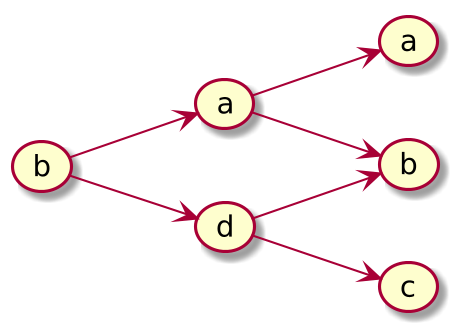
\includegraphics[width=0.2\linewidth]{graph1.png}
\caption{\label{}Graf zależności dla danych testowych 1.}
\end{figure}


\begin{figure}[H]
\centering
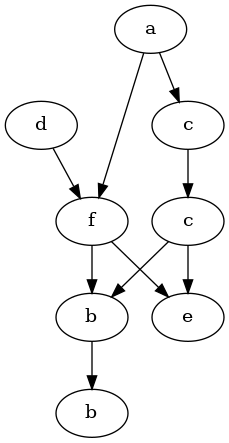
\includegraphics[width=0.25\linewidth]{graph2.png}
\caption{\label{}Graf zależności dla danych testowych 2.}
\end{figure}
\section*{Wnioski}
\label{sec:orgf73a188}
Wyniki algorytmów teorii śladów są zgodne z podanymi wynikami dla danych testowych.
W obu przypadkach poprawność potwierdza również fakt, że niezależnie od sposobu
obliczenia postać normalna Foaty jest identyczna.
\section*{Bibliografia}
\label{sec:org260dfb0}
\begin{itemize}
\item \href{https://www.researchgate.net/publication/280851316\_Partial\_Commutation\_and\_Traces}{Volker Diekert, Yves Metivier : Partial Commutation and Traces}
\item \href{https://graphviz.org/doc/info/lang.html}{Dot Language Documentation}
\end{itemize}
\end{document}
